\chapter{Vendetta in SOL maggiore}

Una lettera è un messaggio scritto di pugno e consegnato nella buchetta di casa per mezzo di un servizio postale.  
Oggi lo si usa poco ma per molte persone ha un significato simbolico, indica l'appartenenza al gruppo di chi non ha dimenticato l'origine terrestre degli esseri umani.  
Inizialmente c'era un po' di diffidenza da parte dei più integralisti, ma poi la percezione che la natura è una e ogni albero vive anche nel complesso dell'intera foresta ha spostato le sensibilità verso una posizione più sostenibile, così in molti si sono convinti che la carta non è il male del mondo ed esprimono con le parole il loro dolore per il pianeta che soffre scrivendole con la matita, sulla carta.  
Una matita fatta di legno sulla carta di cellulosa.  
Parole che sanno di albero che vengono spedite a destinatari incaricati di caricarsi il peso dell'angoscia.

\par\medskip
Laura è seduta sulla poltroncina degli ospiti che sta aiutando l’amica a sbrigare un po’ della corrispondenza, visto che lei è impegnata in faccende che la coinvolgono molto di più.

\par\medskip
\begin{center}
  \includegraphics[width=.55\linewidth]{image1.png}
\end{center}

\begin{verse}\itshape
«Cara Caterina,\\
ti scrivo con le mani sporche di terra e il cuore in fiamme.\\
Ogni giorno mi sveglio con l’ansia che il cielo sia un po’ più basso,\\
che il vento porti con sé un alto grido soffocato di una specie che non c’è più.\\
Eppure continuo a lottare, perché se ci sei tu,\\
tu che hai il coraggio che io non ho…»
\end{verse}

«Vuoi che continui, Cate? Non mi sembra giunga nulla di nuovo alla discussione…»

«Ma sì dai, mi sembra così angosciata, poverina…»

\par\medskip
Caterina è a pochi decimetri da Laura, davanti all’armadio.

\par\medskip
\begin{center}
  \includegraphics[width=.6\linewidth]{image3.png}
\end{center}

Caterina è proprio lì davanti che sceglie i vestiti da mettere in valigia.

Laura riprende, ma il settanta per cento di ciò che legge le sfugge, perché la sua attenzione è catturata dai movimenti mimetici di Alice, seduta sul letto di fronte a lei.

Un viaggio difficile da organizzare, tra biglietti introvabili, alberghi al completo, impegni precedenti e consegne da rispettare sul lavoro.  
Mancano trentasei ore al volo che la condurrà negli Stati Uniti ed è quasi tutto a posto, ma Caterina non sa che sua sorella le sta cucinando una bella vendetta da gustare calda anziché fredda.

Lei se ne va a New York e la lascia a casa con suo padre e sua madre, proprio ora che potrebbero passare una settimana insieme.  
Certo, Alice comprende che il lavoro è importante. Infatti, se fosse solo per quello, non le brucerebbe così tanto.

Ma il problema non è il lavoro. In realtà, lei ci va per Mark.  
Figurati, se non ci fosse lui, avrebbe sicuramente preferito passare l’estate con lei.  
In fondo, di corsi di aggiornamento ce ne sono tanti, nel mondo.  
No, lei lo sa che è per Mark.

\par\medskip
Così, tranquilla, con il suo PC in mano, a gambe incrociate sul letto, mostra uno sguardo innocente.

Vediamo di vedere dove è seduta. Disegniamo anche il letto e, visto che ci siamo, anche la scrivania.  
Dalla camera di una ragazza si può capire molto di lei:

\par\medskip
\begin{center}
  \includegraphics[width=.6\linewidth]{image2.png}
\end{center}

Eccola qui.  
Uno spazio ampio al centro con i mobili accostati verso le pareti, Caterina preferisce l'essere all'apparire.  
La stanza ha tre poli, come i quark: uno per il lavoro, uno per il relax e uno per riposare.  
Che carina, è proprio ordinata.

\par\medskip
Ma torniamo ad Alice.  
Laura le si avvicina per sbirciare cosa sta facendo, ma Alice, con una piccola rotazione, si sottrae al suo sguardo.

«Scusami, sai!» la rimprovera dell'indiscrezione.  
Poi incolla il testo nella sezione \textit{Lyrics} di Suno:

\par\medskip
\textbf{Lyrics}
\begin{quote}\itshape
She leaves and I stay\\
like a folder left open\\
half full, half erased\\
I blink, and she’s already gone
\end{quote}

«Qui capirai quanto ci sono rimasta male…»

\par\medskip
\textbf{Style Description}
\begin{quote}\itshape
Bilingual emotional synth-pop with ambient textures, cinematic flow, and AI female vocals.\\
Slow build. Glitchy, dreamlike, bittersweet. Like diary pages sung in code.
\end{quote}

«Lascia da perdere, è arrabbiata con me.»

«Non sono arrabbiata, solo che voglio finire una cosa.»

«Ha ragione, sono io che sono troppo curiosa.  
Però si è fatta un po’ tardi, è ora che vado a prendere Valentina.»

«No, aspetta solo un attimo, ti prego.»

«Ora la scarico, colleghiamo le casse e voilà!»

\par\medskip
Le note di pianoforte sintetico arpeggiano velocemente una nenia in Sol maggiore.  
Poi, con un respiro sussurrato, inizia il primo verso:

\par\medskip
\textbf{Verse 1}
\begin{quote}\itshape
She leaves and I stay\\
like a folder left open\\
half full, half erased\\
I blink, and she’s already gone
\end{quote}

Questa è la scena prima della crisi…

\par\medskip
\begin{center}
  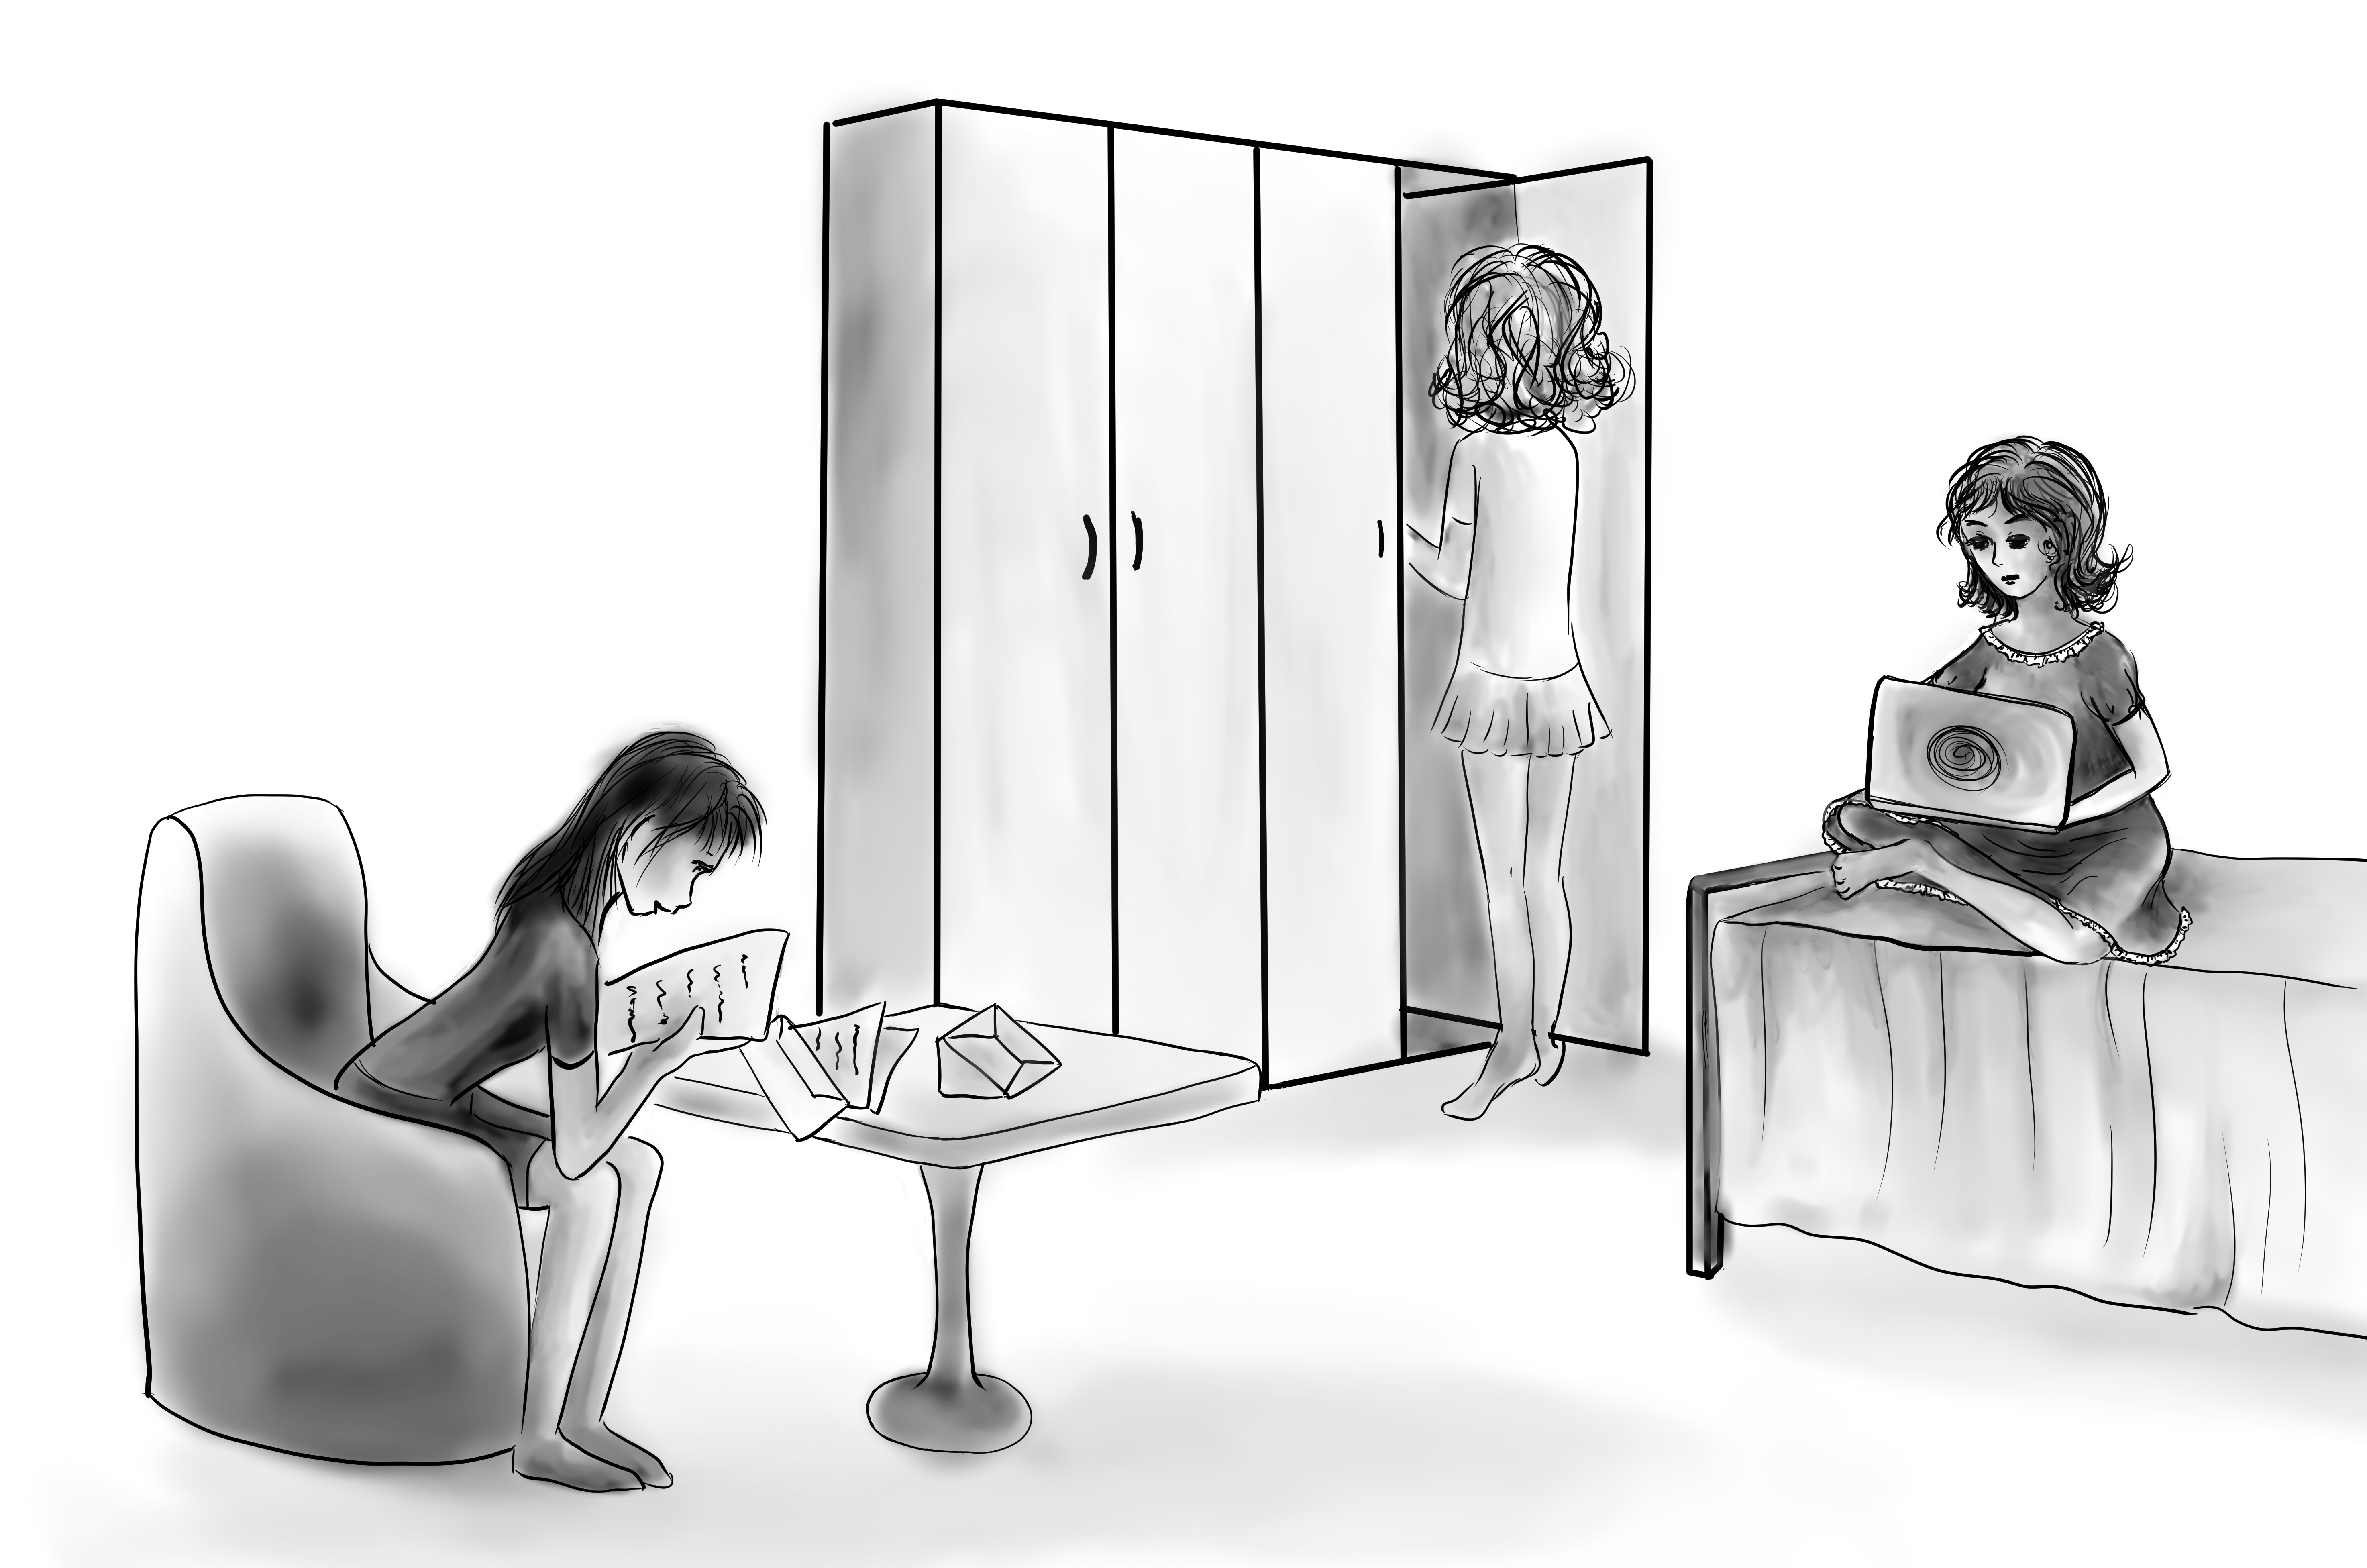
\includegraphics[width=.6\linewidth]{ccsf.png}
\end{center}

\textbf{Verse 2}
\begin{quote}\itshape
She goes to New York\\
I stay with a lamp shaped like a heart\\
plastic love, three settings\\
warm, cold, ambient — mine is blinking
\end{quote}

«E qui voglio vederti piangere!»

\begin{quote}\itshape
I'm not angry, I'm just here
\end{quote}

Una lacrima solca il viso di Caterina, che a stento simula tranquillità continuando a ordinare le cose da mettere in valigia.

«Certo che le semplifichi proprio la partenza, tu.»

Caterina appoggia l’asciugacapelli e si avvicina alla sorella per abbracciarla.

«Non ci provare!» le urla.

Caterina non reagisce. È abituata.  
Alice si libera le ginocchia dal PC e lo poggia sul letto.

«Io esco, mangio qualcosa con le ragazze.»

Caterina si asciuga gli occhi.

«Va bene, ma a casa per le dieci. È l’ultima sera che passiamo insieme.»

«Devo andare anch’io, Cate.»

«Va bene Laura, grazie di essere venuta.»

«Ciao Cate. Ciao Alice.»

Prima di chiudere la porta, Laura ha un attimo di esitazione.  
C’era ancora una cosa, anzi, il motivo principale per cui aveva raggiunto Caterina.

«Ma non sai ancora nulla del visto!»

«Non preoccuparti, Laura. Vedrai che non ci saranno problemi.  
In ogni caso, se ci fossero difficoltà ti chiamo.»

Saluta l’amica con un bacio e corre a prendere Vale.  
Per fortuna manca ancora qualche anno alla sua adolescenza.
